%!TEX root = ../thesis.tex

\section{Tau Decays}\label{tauDecays}
The $\tau$-lepton is the only lepton heavy enough to decay into hadrons. It is an ideal candidate to perform a QCD analysis at low to intermediate energies\footnote{At high energies we have no valid theory because $\alpha_s>>1$ for high-energies.}, extracting and probing Standard model parameters like the strong coupling $\alpha_s$. Due to it's W-Boson mediator it allows a study of the $q\bar q$ vector and axial vector current, whereas $e^+e^-\to\gamma^*\to (hadrons)$ scattering only covers the vector ones.
For the tree level of the SM the tau decays into a $\nu_\tau$ neutrino and a W-Boson, which then decays into either $(\nu_\mu, \mu)$ and $(\nu_e, e)$ lepton pairs or $(\bar u, d)$, and $(\bar u, s)$ quark pairs, as illustrated in Figure \ref{fig:tauDecay}. Other quark pair generation is forbidden either due to the $\tau$-mass of 1776.86 MeV \cite{Olive2014} or the confinement of weak isospin ($T_3$)\footnote{E.g. the $(\bar d, u)$ pair would lead to ($\tau \to \nu_\tau + \bar d + u$), which represents an inequality in terms of weak isopsin conservation ($-1/2 \neq +1/2 + 1/2 - 1/2$).} Due to color confinement\footnote{Quarks have never been seen as single particle, but only in compounds as mesons or baryons.} the detected quark pairs are hadrons (pions, $\rho$ mesons, kaons and others).

\begin{figure}[h]
	\centering
	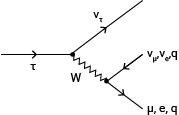
\includegraphics{img/tauDecay.png}
	\caption{Standard Model $\tau$ decays.}
	\label{fig:tauDecay}
\end{figure}

The data is gathered via the ALEPH experiment in CERN and expressed through the ratio
\begin{equation}
  R_\tau = \frac{\mathcal{B}_\tau}{\mathcal{B}_{e^-}} = \frac{\Gamma(\tau^- \to \text{hadrons}^- \nu_\tau)}{\Gamma(\tau^- \to e^- \bar \nu_e \nu_\tau)},
\end{equation}		
which can be connected to the vacuum polarization $\Pi(s)$ of the W-Boson\footnote{Also refered to as the weak current two-point correlation function.}. $\mathcal{B}_\tau$ and $\mathcal{B}_{e^-}$ are the branching fractions of the non strange hadronic and electronic decays and the $\Gamma$s the respective decay rates.

Our aim is to match the experimental data with a theory model in a computer program to analyse and extract parameters of the SM. Therefore we will start connecting the experimental data with quantum field theory. Then describe the needed theory and experimental sides in detail. And lastly discuss the results.

\newpage

\section{Theory}
Starting point of our analysis will be the definition of the vector and axial vector QCD correlator
\begin{equation}
	\Pi_{\mu\nu, ij}^{V/A} (p) \equiv i \int \diff x e^{ipx} \langle \Omega | T \{ J_{\mu, ij}^{V/A} (x) J_{\nu, ij}^{V/A}(0)^\dagger\} | \Omega \rangle,
\end{equation}
with $| \Omega \rangle$ being the physical vacuum and $i,j$ representing the light quark flavours: up, down and strange\footnote{As mentioned before, due to it's mass the $\tau$-lepton cannot decay into the heavier quarks top, bottom and charm.}. The V and A currents are given by
\begin{equation}
	J_{\mu,ij}^{V/A}(x) = [ \bar q_j \gamma_\mu (\gamma_5) q_i](x). 
\end{equation}
The before introduced correlator can be decomposed in several ways starting by the standard longitudinal and transversal decomposition (omitting the flavour indices $i,j$ from now on, if not necassary):
\begin{equation} \label{eq:CorrelatorSpinDecomposition}
	\begin{split}
		\Pi_{\mu\nu}(p)^{V/A} &= (p_\mu p_\nu - g_{\mu\nu} p^2) \Pi^{V/A,(1)}(p^2) + p_\mu p_\nu \Pi^{V/A,(0)}(p^2) \\
		&= (p_\mu p_\nu - g_{\mu\nu}p^2) \Pi^{V/A, (1+0)}(p^2) + g_{\mu\nu} p^2 \Pi^{V/A, (0)}(p^2)
	\end{split}
\end{equation},
where the upper indice $(1)$ denotes the transversal contribution and $(0)$ the longitudinal one. Besides the Lorentz decomposition, the currents contributin to hadronic $\tau$ decays can also be decomposed according to their light quark flavour content:
\begin{equation}
	\Pi_{V/A}^{(J)}(s) = |V_{ud}"^2 \left[ \Pi_{ud}^{V,(J)}(s) + \Pi_{ud}^{A,(J)}(s) \right] + |V_{us}|^2 \left[\Pi_{us}^{V,(J)}(s) + \Pi_{us}^{A,(J)}(s) \right], 
\end{equation}
with $V_{ij}$ being the corresponding elemtns of the Cabibbo-Kobayashi-Maskawas (CKM) quark-mixing matrix.
Another useful decomposition of the V (A) correlator is the separation of vector (axial vector) and scalar (pseudoscalar) components
\begin{equation} \label{eq:CorrelatorVectorScalarDecomposition}
	\begin{split}
	\Pi_{\mu\nu}^{V/A}(p) &= (p_\mu p_\nu - g_{\mu\nu} p^2)\Pi^{V/A} (p^2) \\
	&+ \frac{g_{\mu\nu}}{p^2}(m_i \mp m_j)^2 \Pi^{S,P)}(p^2) + g_{\mu\nu} \frac{m_i \mp m_j}{p^2} [ \langle \bar q_i q_i \rangle \mp \langle \bar q_j q_j\rangle ].
	\end{split}
\end{equation}	
This implies the following relations between the Lorentz scalar function of Eqs. \eqref{eq:CorrelatorSpinDecomposition} and \eqref{eq:CorrelatorVectorScalarDecomposition}
\begin{align}
	s^2 \Pi^{V/A,(0)} (p^2) &= (m_i \mp m_j)\Pi^{S,P}(p^2) + (m_i \mp m_j)[\langle \bar q_i q_i \rangle \mp \langle\bar q_j q_j \rangle], \\
	\Pi^{V/A}, (1+0) (p^2) &\equiv \Pi^{V/A,(1)}(p^2) + \Pi^{V/A, (0)}(p^2) = \Pi^{V/A}(p^2).
\end{align}
Consequently, in the chiral limit ($m_i \to 0$) the longitudinal (Spin-0) component, proportional to the quark masses, vanishes.
With these definitions one can then derive the inclusive decay ratio:
\begin{equation}
	\label{eq:tauDecayRatio}
	R_\tau = 12 \pi S_{EW} \int_0^{m_\tau^2} \frac{\diff s}{m_\tau^2} \left(1 - \frac{s}{m_\tau^2} \right)^2 \left[ \left( 1 + 2 \frac{s}{m_\tau^2} \right) \Im \Pi^{(T)} (s) + \Im \Pi^{(L)} (s) \right],
\end{equation}
where $S_{EW}$ is an electroweak correction factor.

With the help of the QCD Sum Rules, more specifically the FESR we can then rewrite the tau decay ratio \eqref{eq:tauDecayRatio} into
\begin{equation}
	\label{eq:tauRatioFESR}
	R_\tau = 6 \pi i S_{EW} \oint_{|s|=m_\tau^2} \frac{\diff s}{m_\tau^2} \left(1 - \frac{s}{m_\tau^2} \right)^2 \left[ \left( 1 + 2 \frac{s}{m_\tau^2} \right) \Im \Pi^{(T)} (s) + \Im \Pi^{(L)} (s) \right].
\end{equation}
Normally, using the FESR, we need to pay attention to the integral, which runs along the real axis where the perturbation theory is not valid anymore. This problems close to the real axis are believed to be caused by duality violations. The normal procedure would be to introduce so called pinched weight function, which vanishes at the real axis. However, in the case of the $\tau$-decay ratio we naturally derived a pinched weight function (App. \ref{app:tauDecayRatio})
\begin{equation}
	w_\tau(s) = \left(1 - \frac{s}{m_\tau^2}\right)\left(1 + 2 \frac{s}{m_\tau^2} \right),
\end{equation}
which introduce a double zero at $s=m_\tau^2$. The sum rules using pinched weight functions are also referred to as pinched weighted finite energy sum rules or pFESR.
It is convenient to rewrite Eq. \eqref{eq:tauDecayFESR} as
\begin{equation}
		\label{eq:tauRatioFESR2}
	R_\tau = 6 \pi i S_{EW} \oint_{|s|=m_\tau^2} \frac{\diff s}{m_\tau^2} \left(1 - \frac{s}{m_\tau^2} \right)^2 \left[ \left( 1 + 2 \frac{s}{m_\tau^2} \right) \Im \Pi^{(T+L)} (s) - \left(2 \frac{s}{m_\tau^2}\right) \Im \Pi^{(L)} (s) \right],
\end{equation}
where we simply reordered the spin composition
\begin{equation}
	\Pi^{(T+L)}(s) = \Pi^{(T)}(s) + \Pi^{(L)}(s).
\end{equation}
Unfortunately the two-points functions $\Pi^{(J)}$ are not RG invariant and contains scale and scheme dependent subtractions constants. Noticing that the decay ratio integral (Eq. \eqref{eq:tauDecayFESR2}) is RG invariant we can define the so called Adler function, which by itself is RG invariant
\begin{equation}
	\label{eq:AdlerTransform}
	D^{(L+T)}(s) \equiv -s \frac{\diff}{\diff s} \left(\Pi^{(L+T)}(s)\right), \quad D^{(L)}(s) = \frac{s}{m_\tau^2} \frac{\diff}{\diff s} \left( s\Pi^{(L)}(s)\right).
\end{equation}
Making use of integration by parts yields
\begin{equation}
	R_\tau = - \pi i \oint_{|s|=m_\tau^2} \frac{\diff s}{s} \left( 1 - \frac{s}{m_\tau^2}\right)^3 \left[ 3\left( 1 + \frac{s}{m_\tau^2}\right) D^{(L+T)}(s) + 4 D^{(L)}(s) \right],
\end{equation}
which can be calculated within QCD.


\subsection{The theoretical description of the correlator $\Pi(s)$}
\subsubsection{The perturbative contribution}
We will perform our analysis in the chiral limit, which cancels the longitudinal part of the two point function $\Pi^{(L)}(s) = 0$\footnote{The longitudinal part is proportional to the quark masses. Hence zero in the limit of zero quark masses}. This leaves us with with the $\Pi_V^{(T+L)}(s)$ component, which can generally be expressed as \cite{Jamin2008}
\begin{equation}
	\Pi^{(T+L)}_V (s) = - \frac{N_c}{12 \pi^2} \sum_{n=0}^{\infty} a_\mu^n \sum_{k=0}^{n+1} c_{nk} L^k,
\end{equation}
with
\begin{equation}
	L\equiv\log\left(\frac{-s}{\mu}\right) \quad \text{and} \quad a_\mu \equiv a(\mu^2) = \frac{a_s(\mu)}{\pi}
\end{equation}
and $\mu$ being the renormalisation scale.
With the help of Eq. \eqref{eq:AdlerTransform} we can rewrite the former expression into terms of the RG invariant Adler function
\begin{equation}
	D_V^{(T+L)} (s) = \frac{N_c}{12 \pi^2} \sum_{n=0}^\infty a_\mu^n \sum_{k=1}^{n+1} k c_{nk} L^{k-1}
\end{equation},
where the coefficients $c_{n,k}$ are given in App. \ref{app:coefficients}.